\documentclass[conference]{IEEEtran}
\IEEEoverridecommandlockouts
\usepackage{cite}
\usepackage{amsmath,amssymb,amsfonts}
\usepackage{algorithm}
\usepackage{algorithmic}
\usepackage{graphicx}
\usepackage{textcomp}
\usepackage{xcolor}
\usepackage{booktabs}
\usepackage{url}
\usepackage{pifont}
\newcommand{\cmark}{\ding{51}}
\newcommand{\xmark}{\ding{55}}

\begin{document}

\title{RF-FilterLLM: Automated RF Filter Design via\\Domain-Specific Fine-Tuning of Large Language Models}

\author{\IEEEauthorblockN{Wenlong Sun}
\IEEEauthorblockA{\textit{School of Electronics and Information} \\
\textit{Hangzhou Dianzi University}\\
Hangzhou, China \\
wenlong@hdu.edu.cn}
}

\maketitle

\begin{abstract}
This paper describes RF-FilterLLM, a framework that automates radio-frequency ladder-filter design by fine-tuning a large language model (LLM) on domain-specific data. We construct a bilingual instruction-tuning dataset, RF-Filter-SFT (25{,}168 samples), covering Chebyshev Type-I lowpass, highpass, and bandpass topologies.  Three data-augmentation pipelines---perturbation-induced reflection (PIR), bidirectional performance prediction (BPP), and sensitivity-guided tuning---are introduced to provide the model with self-diagnostic and reverse-engineering training signal.  Using QLoRA~\cite{qlora} on a single RTX~4090 (3.83\,M trainable parameters, 9.4\,h), the fine-tuned model raises filter-order prediction accuracy from 19.5\% to 83.4\% while maintaining 100\% JSON-format compliance and near-zero numerical error.  A closed-loop agent that couples the model with Keysight ADS via ABCD-matrix sensitivity analysis~\cite{matthaei} converges within two iterations in practice.  Ablation experiments show that na\"ive fine-tuning on unaugmented data actually \emph{lowers} accuracy below the untuned baseline, underscoring the importance of the proposed data pipelines.
\end{abstract}

\begin{IEEEkeywords}
Large language model, RF filter design, domain-specific fine-tuning, instruction tuning, EDA automation, closed-loop agent
\end{IEEEkeywords}

%=====================================================================
\section{Introduction}
%=====================================================================

Lumped-element RF filters remain a core building block in receiver front-ends, transmitters, and frequency-multiplexing networks.  Designing such a filter involves (i)~computing the minimum order~$N$ that satisfies a set of nonlinear constraints on cutoff frequency~$f_c$, stopband edge~$f_s$, passband ripple~$L_r$, and stopband attenuation~$L_A$; (ii)~synthesizing prototype element values; and (iii)~validating the design through electromagnetic or circuit simulation.  Steps~(i) and (iii) are typically iterative and require considerable microwave-engineering expertise.

Several recent studies have applied LLMs to electronic-design-automation (EDA) workflows.  WiseEDA~\cite{wiseeda} uses GPT-4 for RF circuit sizing, ChipChat~\cite{chipchat} explores conversational HDL generation, and ChipGPT~\cite{chipgpt} investigates prompt-driven digital design.  All three rely on closed-source APIs and do not perform quantitative design-accuracy evaluation; none addresses multi-band filter synthesis.

This paper presents RF-FilterLLM, a locally deployable framework that fine-tunes an open-source LLM for multi-band Chebyshev ladder-filter design.  The main contributions are:
\begin{itemize}
\item A bilingual instruction-tuning dataset (RF-Filter-SFT, 25{,}168 samples across LPF/HPF/BPF) with three task-specific augmentation pipelines and a missing-parameter completion mechanism.
\item A QLoRA training recipe that adapts the model on a single consumer GPU in 9.4\,h, raising order-prediction accuracy from 19.5\% to 83.4\%.
\item A unified frequency-transformation scheme enabling one model to cover three filter bands.
\item A sensitivity-guided reflective agent that pairs the LLM with Keysight ADS through ABCD-matrix perturbation analysis for closed-loop design refinement.
\end{itemize}

%=====================================================================
\section{Methodology}
%=====================================================================

Fig.~\ref{fig:arch} shows the three-stage pipeline of RF-FilterLLM: (1)~dataset construction with task-specific augmentation, (2)~parameter-efficient fine-tuning~\cite{lora,qlora} of an open-source LLM backbone, and (3)~closed-loop validation via an EDA-coupled agent.  The fine-tuned model is referred to as \emph{RF-FilterLLM} throughout.

\begin{figure}[t]
\centering
% TODO: Replace with actual architecture figure
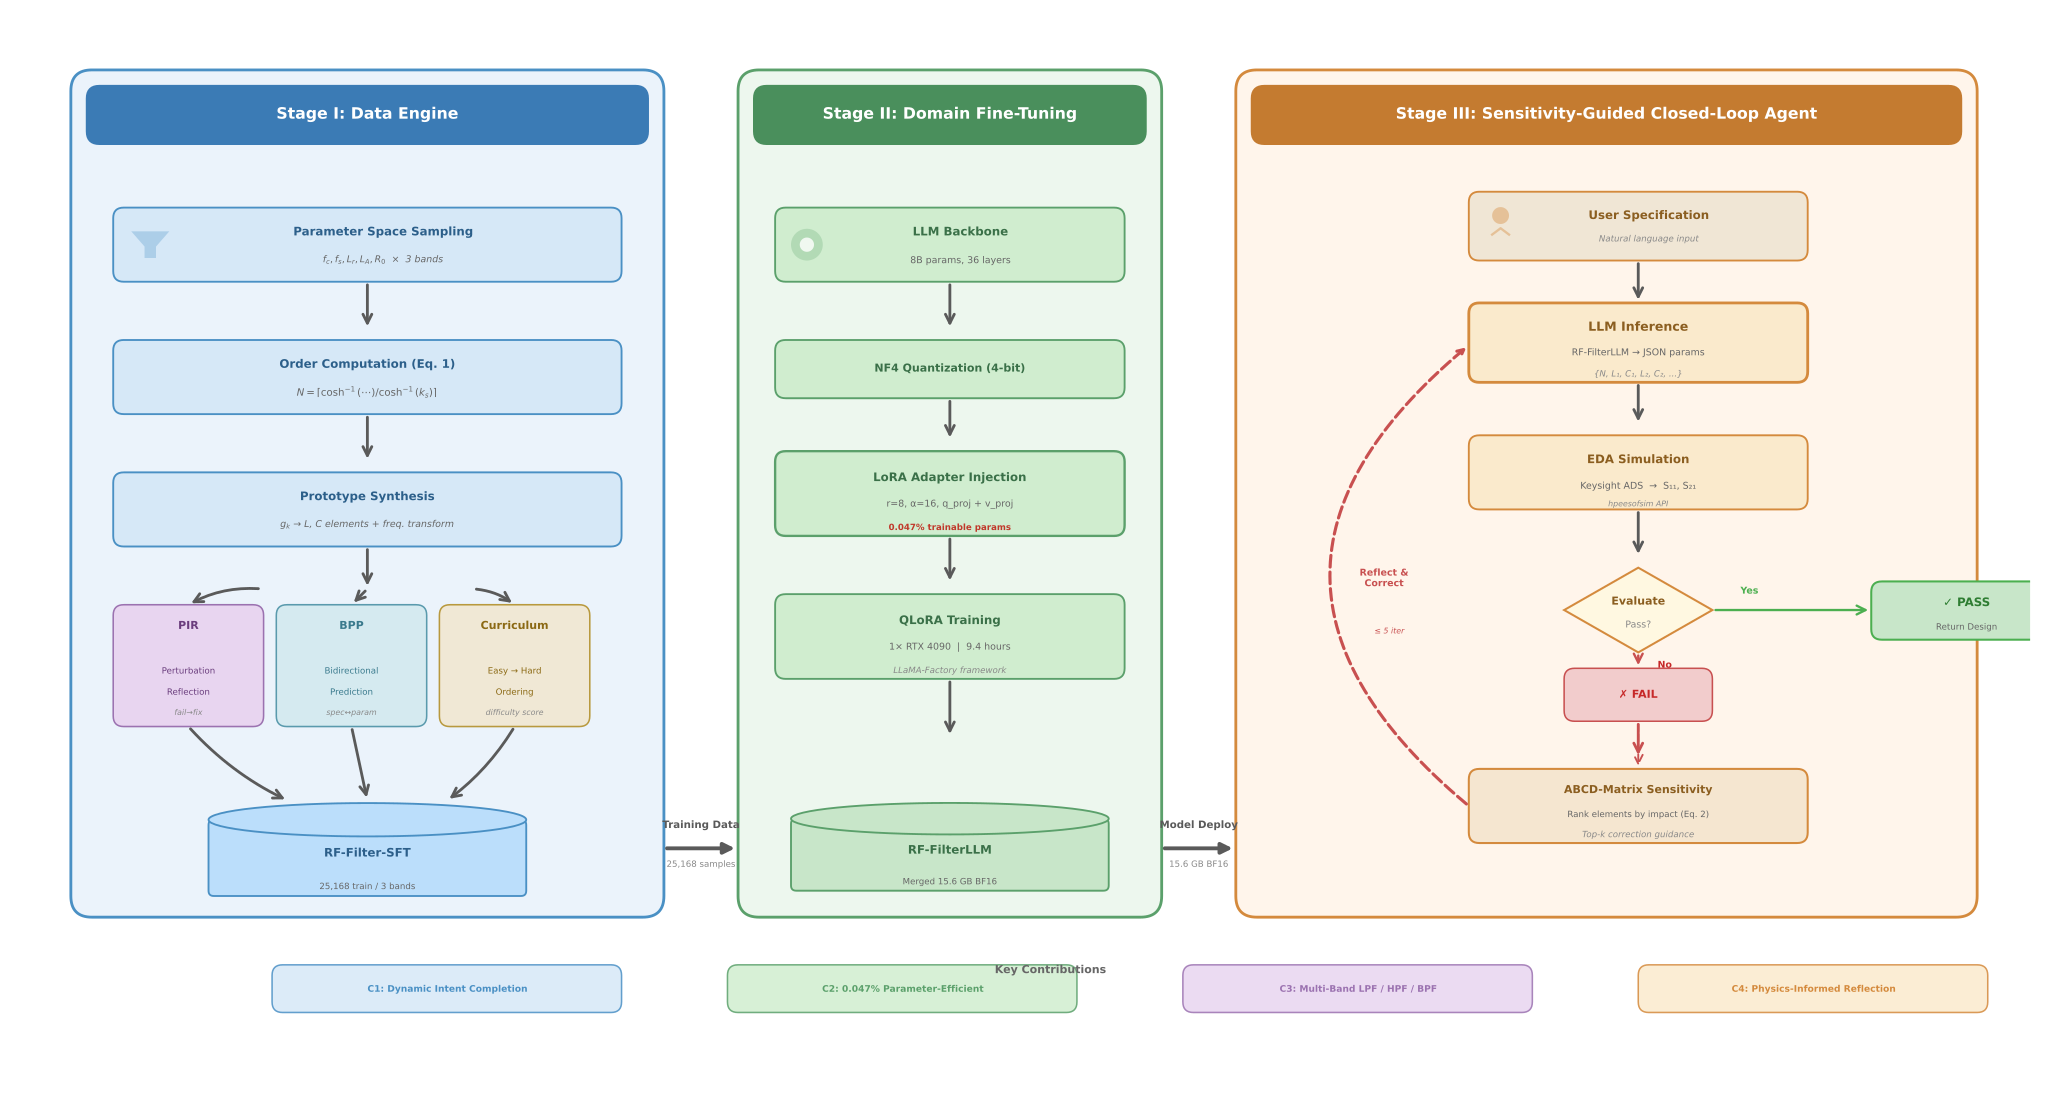
\includegraphics[width=\columnwidth]{figures/architecture.pdf}
\caption{RF-FilterLLM framework overview. Three augmentation pipelines enrich the training data; parameter-efficient fine-tuning yields the domain-adapted model; a sensitivity-guided agent closes the loop with EDA simulation.}
\label{fig:arch}
\end{figure}

\subsection{Dataset Construction and Augmentation}

The RF-Filter-SFT dataset focuses on Chebyshev filters across three bands (LPF, HPF, BPF), with specifications sampled from $f_c\!\in\![100\text{M},3\text{G}]$\,Hz, $k_s\!=\!f_s/f_c\!\in\![1.2,3.0]$, $L_r\!\in\![0.01,1.0]$\,dB, $L_A\!\in\![20,60]$\,dB, and $R_0\!\in\!\{50,75,100\}\,\Omega$. For Chebyshev filters, the required order is:
\begin{equation}
N = \left\lceil \frac{\cosh^{-1}\!\left(\sqrt{(10^{L_A/10}\!-\!1)/(10^{L_r/10}\!-\!1)}\right)}{\cosh^{-1}(k_s)} \right\rceil
\label{eq:order}
\end{equation}
Each sample is formatted as a multi-turn conversation~\cite{ouyang} enforcing strict JSON output. A \emph{dynamic intent completion} mechanism triggers follow-up questions when critical parameters are absent (3.9\% of samples). Table~\ref{tab:dataset} summarizes the dataset statistics.

\begin{table}[t]
\centering
\caption{RF-Filter-SFT Dataset Statistics}
\label{tab:dataset}
\begin{tabular}{lccccc}
\toprule
Split & Samples & LPF & HPF & BPF & ZH:EN \\
\midrule
Train & 25,168 & 40.3\% & 25.7\% & 30.1\% & 82.6:17.4 \\
Val   & 1,415  & 37.8\% & 28.9\% & 30.1\% & 82.5:17.5 \\
Test  & 1,372  & 41.9\% & 29.4\% & 24.7\% & 83.3:16.7 \\
\midrule
\textbf{Total} & \textbf{27,955} & & & & \\
\bottomrule
\end{tabular}
\end{table}

Three augmentation pipelines supplement the base data.  \textbf{Perturbation-induced reflection (PIR)} creates multi-turn ``fail$\to$diagnose$\to$fix'' training examples: controlled deviations (order reduction, frequency drift, excessive ripple) are injected into correct designs, and a rule-based engine generates quantitative diagnostic chains.  Every corrected design is re-verified through a secondary simulation pass.  \textbf{Bidirectional performance prediction (BPP)} adds reverse-direction tasks---predicting performance metrics from given element values, and choosing between two candidate designs according to a minimum-order criterion.  \textbf{Curriculum-ordered training}~\cite{curriculum} ranks samples by a composite difficulty score that weights order complexity, parameter extremity, dialogue depth, and band type, with intra-bucket shuffling to avoid degenerate ordering.

\subsection{Multi-Band Filter Synthesis}

All filters in this work adopt the \textbf{Type-I ladder topology}~\cite{matthaei}: element~$g_1$ is a series inductor, $g_2$ a shunt capacitor, and so on in alternation (Fig.~\ref{fig:arch}).  The Type-II dual (shunt-first) is not used; choosing a single canonical form simplifies the dataset and avoids topology ambiguity in the training signal.

Starting from the Chebyshev lowpass prototype, three bands are realized through standard frequency transformations~\cite{pozar,matthaei}.  For LPF, the prototype undergoes impedance and frequency denormalization.  For HPF, each series inductor is replaced by a series capacitor and each shunt capacitor by a shunt inductor ($L\!\leftrightarrow\!C$ inversion).  For BPF, a narrowband transformation with fractional bandwidth $\delta\!=\!\Delta f/f_0$ converts every prototype element into a series- or shunt-resonator pair, expanding the parameter space from 2D (LPF/HPF) to 5D and making BPF the most challenging prediction target.

A deliberate design choice separates \emph{engineering judgment} from \emph{numerical synthesis}: the LLM predicts the filter order~$N$ and high-level specification parameters, while the physical element values ($L_k$, $C_k$) are computed deterministically from the Chebyshev prototype via classical $g_k$-to-component formulas~\cite{matthaei,pozar}.  This division exploits the LLM's strength at discrete, specification-level reasoning while avoiding the well-known difficulty of regressing precise floating-point values, and guarantees electrical correctness of the resulting ladder network by construction.

\subsection{Sensitivity-Guided Reflective Agent}

The closed-loop agent integrates RF-FilterLLM with Keysight ADS simulation. Given a user specification, the model generates initial filter parameters in JSON format. If the simulated response fails to meet performance criteria, element-wise sensitivity is computed via ABCD-matrix perturbation:
\begin{equation}
S_{x_i}^{m} = \frac{m(x_i(1\!+\!\delta)) - m(x_i)}{m(x_i) \cdot \delta},\quad \delta = 1\%
\label{eq:sens}
\end{equation}
Elements are ranked by aggregate impact score and the resulting report is fed back into the LLM prompt, directing correction toward the most influential components~\cite{reflexion}. This narrows the search space from $\mathcal{O}(N)$ to $\mathcal{O}(k)$ ($k\!\ll\!N$), enabling convergence within five iterations at most. Algorithm~\ref{alg:agent} summarizes this process.

\begin{algorithm}[t]
\caption{RF-FilterLLM Closed-Loop Design}
\label{alg:agent}
\begin{algorithmic}[1]
\REQUIRE Specification $S$, max iterations $T$, pass criteria $E$
\ENSURE Validated design $P^*$
\STATE $P \leftarrow \text{RF-FilterLLM.generate}(S)$
\FOR{$t = 1$ to $T$}
  \STATE $R \leftarrow \text{ADS.simulate}(P)$
  \IF{$\text{evaluate}(R, E) = \text{PASS}$}
    \RETURN $P, R$
  \ENDIF
  \STATE $\sigma \leftarrow \text{ABCD\_sensitivity}(P)$ \COMMENT{Eq.~\eqref{eq:sens}}
  \STATE $P \leftarrow \text{RF-FilterLLM.reflect}(P, R, \sigma)$
\ENDFOR
\RETURN $P, R$
\end{algorithmic}
\end{algorithm}

%=====================================================================
\section{Experiments}
%=====================================================================

\subsection{Results and Ablation}

We evaluate RF-FilterLLM on 199 test samples (175~full, 8~followup-Q, 16~followup-R) using filter-order prediction accuracy ($\text{Acc}_N$) as the core metric. Table~\ref{tab:ablation} presents a three-way comparison: (1)~the untuned backbone, (2)~fine-tuning on $\sim$11k uncleaned samples without augmentation (QLoRA-Early), and (3)~RF-FilterLLM with our full pipeline.

\begin{table}[t]
\centering
\caption{Three-Way Ablation Study}
\label{tab:ablation}
\begin{tabular}{lccc}
\toprule
Metric & No FT & QLoRA-Early & \textbf{Ours} \\
\midrule
Order Acc. (overall) & 19.5\% & 12.6\%\,$\downarrow$ & \textbf{83.4\%} \\
\quad-- LPF & 26.3\% & 7.9\% & \textbf{98.6\%} \\
\quad-- HPF & 23.3\% & 10.0\% & \textbf{98.2\%} \\
\quad-- BPF & 0.0\% & 26.3\% & \textbf{47.1\%} \\
Follow-up Ask Rate & N/A & 0.0\% & \textbf{25.0\%} \\
Multi-turn Order Acc. & N/A & 0.0\% & \textbf{75.0\%} \\
\bottomrule
\end{tabular}
\end{table}

RF-FilterLLM achieves 83.4\% overall order accuracy with 100\% JSON compliance and 100\% type/band accuracy. LPF (98.6\%) and HPF (98.2\%) are near-perfect; BPF (47.1\%) lags behind, consistent with its larger parameter space. Na\"ive fine-tuning on the uncleaned dataset \emph{lowers} order accuracy to 12.6\%---below the untuned baseline of 19.5\%.  Adding PIR, BPP, and curriculum ordering recovers and exceeds the baseline by +63.9 percentage points, indicating that the augmentation pipelines are the primary source of the performance gain.

Fig.~\ref{fig:scatter} visualizes per-sample predictions across all 175~test instances: LPF and HPF cluster tightly along the diagonal, whereas BPF shows a systematic under-prediction pattern.  Fig.~\ref{fig:sparam} translates this into RF consequences for a concrete example ($f_c\!=\!1$\,GHz, $f_s\!=\!2$\,GHz, $L_r\!=\!0.1$\,dB, $L_A\!=\!30$\,dB, requiring $N_{\min}\!=\!5$).  Predicting $N\!=\!4$ yields only 23\,dB of stopband rejection---7\,dB short of the specification---and $N\!=\!3$ fails by 18\,dB.  In contrast, the correct $N\!=\!5$ exceeds the target with 35\,dB.  In closed-loop testing, the reflective agent converged in \textbf{2~iterations}: first-pass simulation returned $S_{11}\!=\!-9.6$\,dB (fail); the model diagnosed insufficient passband matching, reduced the ripple specification from 0.5 to 0.25\,dB, and the second pass achieved $S_{11}\!=\!-12.4$\,dB (pass).

\begin{figure}[t]
\centering
\includegraphics[width=\columnwidth]{figures/order_scatter.pdf}
\caption{Per-sample order-prediction results (175~test instances). Points on the dashed diagonal are correct predictions. Red-edged markers indicate errors. BPF (triangles) shows systematic under-prediction.}
\label{fig:scatter}
\end{figure}

\begin{figure}[t]
\centering
\includegraphics[width=\columnwidth]{figures/sparam_spec_impact.pdf}
\caption{Impact of order-prediction error on a Chebyshev LPF ($f_c\!=\!1$\,GHz, $L_A\!=\!30$\,dB, $N_{\min}\!=\!5$). Predicting $N\!=\!4$ falls 7\,dB short of the spec; $N\!=\!3$ misses by 18\,dB.}
\label{fig:sparam}
\end{figure}

\begin{figure}[t]
\centering
\includegraphics[width=\columnwidth]{figures/closed_loop_convergence.pdf}
\caption{Closed-loop convergence in 2~iterations. Left: $S_{11}$ improves from $-9.6$\,dB (fail) to $-12.4$\,dB (pass). Right: passband ripple is halved from 0.50 to 0.25\,dB after reflective self-correction.}
\label{fig:closedloop}
\end{figure}

\subsection{Comparison with Related Work}

Table~\ref{tab:compare} compares RF-FilterLLM with published LLM-based EDA methods.  To our knowledge, this is the first open-source, fine-tuned LLM that covers multiple filter bands and provides quantitative order-accuracy evaluation together with a closed-loop simulation agent.

\begin{table}[t]
\centering
\caption{Comparison with Existing Methods}
\label{tab:compare}
\setlength{\tabcolsep}{3pt}
\begin{tabular}{lcccccc}
\toprule
Method & FT? & Bands & Acc$_N$ & Local & Loop & Cost \\
\midrule
WiseEDA~\cite{wiseeda} & \xmark & LPF & N/R & \xmark & PSO & API \\
ChipChat~\cite{chipchat} & \xmark & N/A & N/A & \xmark & \xmark & API \\
ChipGPT~\cite{chipgpt} & \xmark & N/A & N/A & \xmark & \xmark & API \\
Baseline & \xmark & 3 & 19.5 & \cmark & \xmark & -- \\
\textbf{RF-FilterLLM} & \cmark & \textbf{3} & \textbf{83.4} & \cmark & \textbf{Refl.} & \textbf{9.4h} \\
\bottomrule
\end{tabular}
\end{table}

%=====================================================================
\section{Conclusion}
%=====================================================================

We described RF-FilterLLM, a framework that fine-tunes an open-source LLM for automated Chebyshev ladder-filter design.  The RF-Filter-SFT dataset (25{,}168 samples), enriched by PIR, BPP, and curriculum-ordered training~\cite{curriculum}, enables QLoRA adaptation~\cite{qlora} that raises order-prediction accuracy from 19.5\% to 83.4\% with full output compliance.  Ablation shows that the augmentation pipelines are essential; without them, fine-tuning actually degrades accuracy below the untrained baseline.  The sensitivity-guided agent pairs the model with Keysight ADS and converges within two iterations.  Future work includes BPF-targeted oversampling, extension to elliptic-filter topologies, and transfer across model architectures.

\section*{Acknowledgment}
This work was supported by the National Natural Science Foundation of China under Grants 62371296 and 62188102, and by the State Key Laboratory of Radio Frequency Heterogeneous Integration (Independent Scientific Research Program No. 2025017-SJTU).

\begin{thebibliography}{00}
\bibitem{wiseeda} Y.~Zhang \emph{et al.}, ``WiseEDA: An LLM-assisted automated design framework for RF circuits,'' \emph{IEEE Trans. Microw. Theory Techn.}, 2024.
\bibitem{chipchat} J.~Blocklove \emph{et al.}, ``Chip-Chat: Challenges and opportunities in conversational hardware design,'' in \emph{Proc. ACM/IEEE DAC}, 2023.
\bibitem{chipgpt} K.~Chang \emph{et al.}, ``ChipGPT: How far are we from natural language hardware design,'' \emph{arXiv:2305.14019}, 2023.
\bibitem{lora} E.~J.~Hu \emph{et al.}, ``LoRA: Low-rank adaptation of large language models,'' in \emph{Proc. ICLR}, 2022.
\bibitem{qlora} T.~Dettmers \emph{et al.}, ``QLoRA: Efficient finetuning of quantized language models,'' in \emph{Proc. NeurIPS}, 2023.
\bibitem{matthaei} G.~L.~Matthaei, L.~Young, and E.~M.~T.~Jones, \emph{Microwave Filters, Impedance-Matching Networks, and Coupling Structures}.\hskip 1em plus 0.5em minus 0.4em Norwood, MA: Artech House, 1980.
\bibitem{pozar} D.~M.~Pozar, \emph{Microwave Engineering}, 4th~ed.\hskip 1em plus 0.5em minus 0.4em Hoboken, NJ: Wiley, 2012.
\bibitem{curriculum} Y.~Bengio \emph{et al.}, ``Curriculum learning,'' in \emph{Proc. ICML}, 2009.
\bibitem{reflexion} N.~Shinn \emph{et al.}, ``Reflexion: Language agents with verbal reinforcement learning,'' in \emph{Proc. NeurIPS}, 2023.
\bibitem{llamafactory} Y.~Zheng \emph{et al.}, ``LlamaFactory: Unified efficient fine-tuning of 100+ language models,'' in \emph{Proc. ACL System Demonstrations}, 2024.
\bibitem{ouyang} L.~Ouyang \emph{et al.}, ``Training language models to follow instructions with human feedback,'' in \emph{Proc. NeurIPS}, 2022.
\end{thebibliography}

\end{document}